\documentclass{article}

\usepackage{xcolor}
\colorlet{dark-cyan}{cyan!75!black}
\newcommand\katja[1]{{\color{dark-cyan}Katja: #1}}

\newcommand\TODO[1]{{\color{red}TODO: #1}}
\newcommand\MAYBE[1]{{\color{blue} #1}}

% if you need to pass options to natbib, use, e.g.:
%     \PassOptionsToPackage{numbers, compress}{natbib}
% before loading neurips_2019

% ready for submission
% \usepackage{neurips_2019}

% to compile a preprint version, e.g., for submission to arXiv, add add the
% [preprint] option:
     \usepackage[preprint]{neurips_2019}

% to compile a camera-ready version, add the [final] option, e.g.:
%     \usepackage[final]{neurips_2019}

% to avoid loading the natbib package, add option nonatbib:
%     \usepackage[nonatbib]{neurips_2019}

\usepackage[utf8]{inputenc} % allow utf-8 input
\usepackage[T1]{fontenc}    % use 8-bit T1 fonts
\usepackage{hyperref}       % hyperlinks
\usepackage{url}            % simple URL typesetting
\usepackage{booktabs}       % professional-quality tables
\usepackage{amsfonts}       % blackboard math symbols
\usepackage{nicefrac}       % compact symbols for 1/2, etc.
\usepackage{microtype}      % microtypography
\usepackage{graphicx}

\title{Win or Learn Fast Proximal Policy Optimization (WoLF-PPO)}

% The \author macro works with any number of authors. There are two commands
% used to separate the names and addresses of multiple authors: \And and \AND.
%
% Using \And between authors leaves it to LaTeX to determine where to break the
% lines. Using \AND forces a line break at that point. So, if LaTeX puts 3 of 4
% authors names on the first line, and the last on the second line, try using
% \AND instead of \And before the third author name.

\author{%
  Dino S.~Ratcliffe\\
  Department of Computer Science\\
  Queen Mary University of London\\
  Mile End, London \TODO{check proper address format} \\
  \texttt{d.ratcliffe@QMUL.AC.UK} \\
  % examples of more authors
  % \And
  % Coauthor \\
  % Affiliation \\
  % Address \\
  % \texttt{email} \\
  % \AND
  % Coauthor \\
  % Affiliation \\
  % Address \\
  % \texttt{email} \\
  % \And
  % Coauthor \\
  % Affiliation \\
  % Address \\
  % \texttt{email} \\
  % \And
  % Coauthor \\
  % Affiliation \\
  % Address \\
  % \texttt{email} \\
}

\begin{document}

\maketitle

\MAYBE{Making claims we haven't proven}

\TODO{Represents a TODO comment}

\begin{abstract}
    We consider learning strategies in fully competitive zero-sum games. There have been two main properties identified as desirable for agents that learn in  such settings. This includes being convergent in self play, where the agent learns a Nash Equilibrium Strategy (NES) and minimizing regret when dealing with opponent agents that are playing a stationary policy. One approach for dealing with these problems is Win or Learn Fast (WoLF), this approach has been shown to converge to NES in self play, as well as playing best response when playing against stationary opponents. In this paper we look to combine the recent advancements in Deep Reinforcement Learning with Win or Learn Fast. In particular - we focus on a policy gradient algorithm, PPO, which has shown excellent empirical performance in multi-agent scenarios (self-play). We present a systematic empirical investigation into whether WoLF can be effectively adapted to this state of the art algorithm, and whether the characteristics of WoLF continue to hold. \MAYBE{We demonstrate that WoLF is able to improve the performance of PPO in multiple environments and give insight into environment properties that help PPO learn a strategy close to the NES.} \katja{Mention key result / insight here.}

  % Many advancements have been made in deep reinforcement learning in recent years, allowing approaches such as Deep Q-Networks (DQN) to learn from the raw game images. These systems can produce better than human play in a range of classic Atari games. We empirically show that combining these approaches allows for better convergence to the NES and best response in multiagent environments with more complex state space representations.
\end{abstract}

\section{Introduction}

\section{Background}

\subsection{Game Frameworks}

\subsubsection{Markov Decision Process} is the framework that is used for dealing with reinforcement
learning in the single agent environment. MDP can be represented by the tuple 
$(\mathcal{S}, \mathcal{A}, \mathcal{T}, \mathcal{R})$ were $S$ is the set of possible
states, $A$ is the set of possible actions, $T$ is a transition function of the form 
$\mathcal{S}\times\mathcal{A}\times\mathcal{S}\rightarrow [0,1]$ that gives a probability
distribution over next states after a given action is performed in a given state. Finally
$R$ represents a reward function of the form $\mathcal{S}\times\mathcal{A}\rightarrow \mathbb{R}$
that returns a reward when a given action is performed on a given state. This framework presents a problem that can be solved by maximising the discounted
future reward with a given discount factor denoted by $\gamma$. All MDPs can be solved
with a stationary deterministic policy, this results in the majority of single agent
RL work focusing on agents that solve this type of problem without much consideration
of how they may perform in a multiagent environment where a deterministic strategy may
not be optimal.

\subsubsection{Matrix Games}

A framework that does deal with multiple agents are matrix games. These games
can be represented by the following tuple $(n, \mathcal{A}_{1...n}, \mathcal{R}_{1...n})$
where $n$ represents the number of agents, $\mathcal{A}_{i}$ represents the actions
available to agent $i$ with $A$ representing the joint action between all agents and 
$\mathcal{R}_{i}$ represents the reward function for agent $i$. It is the reward 
function that gives this framework its name as it can easily be represented as 
$n$ set of matrices. Matrix games have a couple of different forms as either zero-sum games or general-sum
games. Zero-sum games are strictly competitive, were if one of the agents receives a
positive reward then the opposing agent receives a negative reward, this can sum to 
either zero or some other constant. General-sum games do not have this constraint and
can even have reward matrices that are identical across agents, resulting in strictly
cooperative games. When considering what solved means for this framework two properties emerge, they are
the Best Response strategy and the Nash Equilibrium. The best response strategy is the optimal strategy against the joint actions of all the
other agents. In the case of playing against a set of stationary opponents there will 
exist a deterministic best response strategy. Nash equilibrium takes this one step further and states that all agents should be playing
a best response against the joint actions of all its respective opponents. This produces
a dynamic where an agent playing the Nash equilibrium can not do better by changing strategy
whilst the other agents are also playing a Nash equilibrium. This does not mean that the
Nash equilibrium is an optimal strategy against all agents however it does provide 
stability by preventing the agent from being exploited by another strategy. Nash equilibrium
have also been proven to exist in all zero-sum games (contain a unique Nash equilibrium) and
all general sum games, making it a very desirable strategy to be able to learn.

\subsubsection{Stochastic Games} is a frame work that combines the Markov Decision Process (MDP) framework and the 
Matrix games framework. It can be seen as a MDP with with multiple agents producing 
a joint action that is used for the transition function and agents reward function. Stochastic games can be seen as the fol owing tuple $(n, \mathcal{S}, \mathcal{A}_{1...n}, 
\mathcal{T}, \mathcal{R}_{1...n})$. This is with $n$ representing the number of agents 
in the game, $\mathcal{S}$ being the set of possible states, $\mathcal{A}_{i}$ being the 
set of actions available to agent $i$, $\mathcal{A}$ represents the set of joint actions, 
$\mathcal{T}$ is a transition function in the form of 
$\mathcal{S}\times\mathcal{A}\times\mathcal{S}\rightarrow [0, 1]$ giving a probability 
distribution over states that result from the joint action $\mathcal{A}$ being performed
on a given state, finally $\mathcal{R}_{i}$ is a reward function for agent $i$ in the form
$\mathcal{S}\times\mathcal{A}\rightarrow \mathbb{R}$. As stochastic games are built on MDP and matrix games both of these are subsets of
stochastic games. A stochastic game with all opposing agents having stationary policies
is identical to a MDP. If the Stochastic game only has one state then it is identical 
to a matrix game. Some of the properties from matrix games also transition over to stochastic games, 
this includes the notion of zero-sum games and general sum games. This also means
that Nash equilibrium strategies exist for stochastic games and this is the strategy
that the original WoLF work and our work is trying to learn.

\katja{best response? discuss other solution concepts if relevant}

\subsection{Properties of Multi-Agent systems}

Within multiagent literature two main properties have
been identified as desirable for any multiagent learning
system.

The first of these properties is rationality, this property requires
the agent to learn a best-response strategy against any agent that 
converges to a stationary policy. This is a relatively easy property to 
obtain, given that stochastic games with an opponent playing a stochastic 
policy can be framed as an MDP. So this means that any agent that can 
solve an MDP is rational by this definition.

The second property dictates that the agent will converge to a stationary policy given 
a stationary agent or a learning agent from a defined class. This class of learning
algorithms is usually defined as consisting of most "useful" algorithms (often restricted
to rational algorithms). In practise this results in most literature focusing on self 
play, however some work has been empirically shown to converge with a small subset of learning 
agents beyond self play. 

The reason that these two rules have been identified as desirable properties for mulitagent
systems to possess is how their relationship relates to the Nash equilibrium. This comes from 
the fact that if both agents are rational and both converge to a stationary policy then they
must have converged to a Nash equilibrium. This can logically be thought through, if both 
agents are guaranteed to play best response to a stationary policy then neither of the agents 
can individually change their strategy in order to increase their payoff. Given this the agents 
must have then converged to a Nash equilibrium.

\section{Related Work}

\subsection{WoLF}

Infinitesimal Gradient Ascent (IGA) has been proven in self play will either converge to a Nash equilibrium,
or the average payoffs over time will converge in the limit to a Nash Equilibrium. This provides an agent
that is both rational and convergent. However this is regarded as a week form of convergence as it may only
converge to the payoff of a Nash equilibrium in expectation. This work was then expanded on with variable
learning rates.

The introduction of a variable learning rate method, Win or Learn Fast (WoLF) looks to extend IGA into a
method that has a stronger notion of converging to a Nash equilibrium. This is done by introducing separate
learning rates for when the agent is winning and when it is losing. The agent is judged to be winning if their
current expected payoff is better than playing the Nash equilibrium. This change has the effect of the winning
agent learning slower and being more "cautious" about updating its strategy until the other agent has learnt 
to counter the new strategy.

This approach does place some strict requirements on what knowledge is needed of the game. The method requires
the player's own payoff matrix to be known and the policy of the opponent agent. It would also need to know
the Nash Equilibrium in order to compute if the agent is currently winning or losing, this however can be 
computed from the known payoffs.

Although the proofs for this method do require knowing detailed information about the environment and opponent,
a practical algorithm has been presented. This method is based on PHC and uses a comparison of the current expected
payoff to the expected payoff of the current average policy. This provides a estimation of the equilibrium policy.

\begin{itemize}
    \item WoLF Guarantees
\end{itemize}

\subsection{PPO}

\subsection{\TODO{more info on Nash learning algorithms}}

\section{Empirical Experiments}

For our empirical results we aimed to highlight the difference between PPO and WoLF-PPO, we have therefore used the same experimental setup and environments form the original WoLF paper, as these were also designed to highlight the advantages of WoLF. We also introduce some weighted variants the the environments to highlight the effect of the entropy term present in PPOs objective function.

\subsection{Matching Pennies}

The first and simplest environment we used is Matching Pennies in both its original form with a uniform random Nash Equilibrium and a weighted form, were the Nash Equilibrium is shifted away from uniform random. The payoff matrices are shown in fig \TODO{Put in fig}. 
Matching pennies is a game were both players pick a side of a coin, either heads or tails, these choices are then reveled simultaneously with one player receiving a point if they match and the other receiving a point if they differ. This results in the Nash Equilibrium being uniform random, if you pick the side of the coin at random then you will win 50\% of the games irrespective of your opponents strategy.

\subsection{Rock Paper Scissors}

Moving up form matching Pennies we used Rock Paper Scissors as our next environment. This game consists of three possible actions that form a cyclic winning pattern, as shown in Fig \TODO{put in fig}.

This environment is of interest because many complex commercial games will have multi-agent scenarios that mimic Rock Paper Scissors [ref]. We again present the standard version of Rock Paper Scissors and a weighted variant to move the Nash Equilibrium away from uniform random. The payoff matrices for these versions can be found in Fig \TODO{put in fig}.

\subsection{Gridworld Soccer}

The final environment that we test the performance of WoLF-PPO on is gridworld soccer. This is a game that consists of two players in a gridworld environment. They are required to score goals by moving into the opponents goal whilst carrying the ball. The agents have 5 actions available, moving in the 4 cardinal directions and the ability to stay in the current position. A tackle is performed when the ball carrier attempts to move onto a space occupied by the opponent. The players moves are submitted simultaneously and then performed in a random order, this gives the game non-determinism. An initial game state is shown in Fig \TODO{put in fig}.

In this environment deterministic polices can be exploited as shown in Fig \TODO{put in fig}. This state requires player A to play a mixed strategy in order to have a chance of scoring, as the other agent could just continue to block the goal if its opponent was player a pure strategy. 

The experiments are designed to address the following research questions. These were selected to align with [ref WOLF paper] to investigate those empirical tasks where WOLF was shown to benefit / be required to solve the task.

Research questions:
\begin{itemize}
    \item RQ 1: Do the properties that WoLF has shown in tabular RL extend to DRL? (with stochastic policies)
    \item RQ 1a: Does PPO empirically converge to best response against stationary stochastic opponents (in repeated matrix fully competitive zero-sum games)?
    \item RQ 1b: Does WoLF-PPO empirically converge to best response against stationary stochastic opponents (in repeated matrix games)?
    \item RQ 1c: Does WoLF-PPO converge more quickly / robustly / with lower variance than PPO converge to best response against stationary stochastic opponents (in repeated matrix games)?
    \item RQ 1d: Do PPO / WoLF-PPO converge to the NE in self-play (in repeated matrix games)? (does one converge more quickly / reliably ... than the other)
    \item RQ 2: Do the above empirically hold in extensive form games?
    \item RQ 3 (optional): How does WoLF-PPO perform empirically against other types of learning opponents (PPO)?
\end{itemize}

\subsection{Matching Pennies}
Addresses RQ 1a,b,c,d

\subsection{Weighted Matching Pennies}
Addresses RQ 1a,b,c,d

\subsection{Rock Paper Scissors}
Addresses RQ 1a,b,c,d

\subsection{Soccer Game}
Addresses RQ2

\section{Results}

\subsection{Matching Pennies}

The results of our experiments on matching pennies provided insight on the ability for PPO and WoLF-PPO to learn the Nash Equilibrium in self play.

Starting with PPO and WoLF-PPO on the standard weighting of matching pennies we can see that both agents stay close to the Nash equilibrium as shown in Fig \TODO{put in fig}. You can see that the variance for PPO is still within X of the Nash equilibrium. In this setting we see that WoLF-PPO does indeed have lower variance than PPO but not by a large margin.

When the learning rate is increased by an order of magnitude as in Fig \TODO{put in fig}, it is apparent that the variance away from the Nash equilibrium increases for both PPO and WoLF-PPO. however WoLF-PPO stays much closer to the Nash equilibrium. We believe that the relatively good performance of PPO in this environment is due to the maximizing of entropy in PPOs objective function. In games such as matching pennies the Nash equilibrium is to play uniform random and thus max entropy. That results in this version of matching pennies having its Nash equilibrium directly optimized in the objective function.

The results for weighted matching pennies demonstrate this by shifting the Nash equilibrium away from the max entropy strategy. In Fig \TODO{put in fig} we can see that PPO now wildly diverges away from the Nash equilibrium strategy, with the variance being larger than when dealing with the non weighted matching pennies. We also see that WoLF-PPO outperforms PPO by a larger amount in this environment, showing the benefit of WoLF-PPO in environments without the Nash equilibrium lying on the max entropy strategy.

\subsection{Rock Paper Scissors}

In Rock Paper Scissors we see very similar results to what we observed in matching pennies. In Fig \TODO{put in fig} we show a sample run of PPO and WoLF-PPO, as shown they both stay close to the Nash equilibrium, as with standard matching pennies the Nash equilibrium lays on the max entropy strategy resulting in relativly good performance from PPO. When increasing the learning rate by an order of magnitude we end up with WoLF-PPO showing reduced varience. This is the same behaviour observed in matching pennies.

We then ran PPO and WoLF-PPO on a weighted version of Rock Paper Scissors. This is to move the Nash equilibrium away from the max entropy policy. In Fig \TODO{put in fig} we show that in this environment WoLF-PPO stays closer to the Nash equilibrium than PPO. This is consistent with the matching pennies results. We also show in Fig \TODO{put in fig} that even when increaing the learning rate by an order of magnitude WoLF-PPO is still able to outperform PPO, the distance from the Nash equilibrium is increased howver nto to the degree of PPO.

\subsection{Gridworld Soccer}

\TODO{Give results using PPO and WoLF PPO, including LR, entropy, WoLF-Ratios and epochs sweeps.}

\section{Conclusion}

Connection with IPD - hysteretic agents ... questions around assessing "winning" or "losing" in more general games

\subsubsection*{Acknowledgments}

Use unnumbered third level headings for the acknowledgments. All acknowledgments
go at the end of the paper. Do not include acknowledgments in the anonymized
submission, only in the final paper.

\section*{References}

References follow the acknowledgments. Use unnumbered first-level heading for
the references. Any choice of citation style is acceptable as long as you are
consistent. It is permissible to reduce the font size to \verb+small+ (9 point)
when listing the references. {\bf Remember that you can use more than eight
  pages as long as the additional pages contain \emph{only} cited references.}
  
\section*{Reproducing Bowling Soccer Experiments}

\TODO{Not sure if this should be in the paper or not, definitely would need to go somewhere else and be shorter}

The outline used for the soccer experiments in the Bowling paper are based on the experiments used to demonstrate Minimax-Q learning. There are however some pieces of information missing between these two sources that makes reproducing the results difficult. 

\subsection*{Experimental Setup}

The main high level detail of the experiment are as follows.

PHC/WoLF-PHC are trained against another agent of the same type for 1 million steps, these agents are then trained for a further 250k steps with there policies being check-pointed at every 50k increment.

This results in 6 polices per player. A set of Q agents are then trained against these stationary polices. This creates a worst case opponent for all the polices that the PHC/WoLF-PHC agents generated. These polices are then evaluated by determining their win rate against the worst case opponent that is able to maximally exploit the agent. The worst win-rate out of the 6 polices per agent is then considered that agents win-rate. The reason for this approach is due to the fact that the agents will circle around and through the Nash equilibrium, by taking a few checkpoints we are able to get an estimation of the furthest point at which the agent is circling the Nash. 

\subsection*{Environment Ambiguity}

The soccer environment itself has some ambiguity. The information that is given includes the rewards for scoring a goal, the size of the pitch, the action space and the possible initial states. The other areas of the environment have varying levels of ambiguity, these include, how tackles function, reward structure for other events, ability to score own goals and the terminal conditions of the game.

\subsubsection*{Tackles}

Tackles in the game are explained in both the original Minimax-Q paper and the Bowling papers on the subject. However there seems to be some discrepancy between the two. In the case of Minimax-Q it seems that when a tackle takes place the agent that has been tackled does not complete their move action, As shown in Fig \ref{fig:minimax-tackle}. However in the Bowling paper Fig \ref{fig:bowling-tackle} appears showing the agent completing its move action after a tackle. 

\begin{figure}
    \centering
    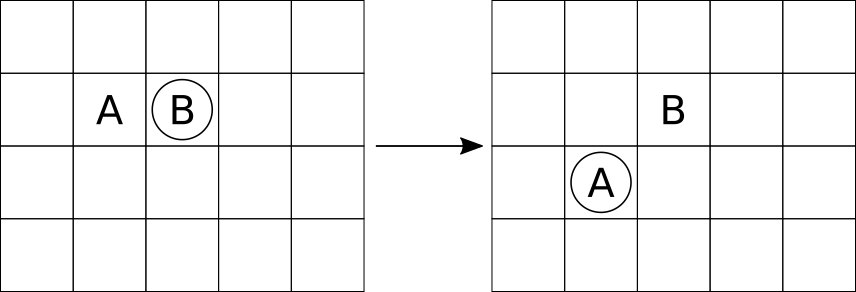
\includegraphics[width=20em]{./Figures/minimax-tackle.png}
    \caption{Tackle as described for Minimax-Q, when A agent moves down and B agent moves left}
    \label{fig:minimax-tackle}
\end{figure}

\begin{figure}
    \centering
    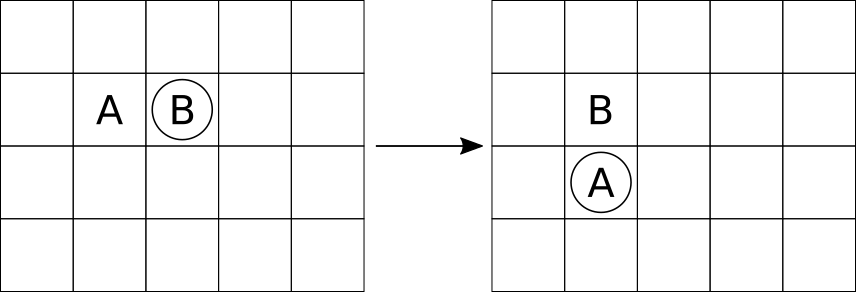
\includegraphics[width=20em]{./Figures/bowling-tackle.png}
    \caption{Tackle as described in Bowling, when A agent moves down and B agent moves left}
    \label{fig:bowling-tackle}
\end{figure}

\subsubsection*{Rewards}

The rewards are given for scoring and conceding goals in the Minimax-Q paper, +1 and -1 respectively. It is not stated what reward is given during drawn games in our experiance this has been a vital setting for training the Q agents against the pretrained PHC/WoLF-PHC agents with no reward resulting in Q agents that find sub optimal local minima but agents that receive a negative reward for draw games improving there average payoff.

\subsubsection*{Terminal Condition}
The terminal condition is a vital piece of information that both the Minimax-Q and Bowling papers leave open to interpretation. In the Minimax-Q paper a terminal condition is given, however this is only stated in the context of evaluating the agents against each other not for training. The terminal condition that is given states that at each time-step there is a probability P(0.1) that the game will terminate at the time-step. It is not stated if this is also the terminal condition for the training stage of the experiment.

\subsection*{Agent Ambiguity}

There are a few ambiguities for both the Q agent opponents and the PHC and WoLF-PHC agents. 

\subsubsection*{Q Agents}

The Q agent is well defined in the Minimax-Q paper however no information on this agent is given in the bowling paper, they do however state that they tried to follow the experimental setup of Minimax-Q as closely as possible, so it is assumed the details given in Minimax-Q were used.

\subsubsection*{PHC/WoLF-PHC}

The policy hill climbing algorithms presented in the Bowling papers do however have ambiguous details. In the short papers PHC is stated to follow and epsilon-greedy policy when selecting actions, this is however incorrect and an epsilon-projection action should be selected. This is fixed in the Bowling thesis.

Another source of ambiguity and the most important is the definition of the learning rates given for the experiments. They are all of the form presented in Equation \ref{eq:lr}. 

\begin{equation}
    \alpha = \frac{1}{10+\frac{t}{500}}\label{eq:lr}
\end{equation}

all of the learning rates follow this pattern and rely on the value of t, however t has different meaning from different publications, these publications are reporting the same results with the same learning rates. In the bowling short papers t is defined to be the visit count of the current state C(s). Whereas in the bowling thesis this has changed to be the count that the given state action pair has been visited C(s, a).



\medskip

\small

[1] Alexander, J.A.\ \& Mozer, M.C.\ (1995) Template-based algorithms for
connectionist rule extraction. In G.\ Tesauro, D.S.\ Touretzky and T.K.\ Leen
(eds.), {\it Advances in Neural Information Processing Systems 7},
pp.\ 609--616. Cambridge, MA: MIT Press.
\end{document}
